% Define document class
\documentclass[twocolumn]{aastex631}

% Custom style defs for this paper
\usepackage{listings}

\lstdefinestyle{bash}{%
    language=bash,
    basicstyle=\ttfamily\footnotesize,
    texcsstyle=*\bf\color{black},
    numbers=none,
    breaklines=true,
    commentstyle=\color{red},
    frame=single
}
\lstdefinestyle{yaml}{%
    basicstyle=\ttfamily\footnotesize,
    texcsstyle=*\bf\color{black},
    numbers=none,
    breaklines=true,
    commentstyle=\color{red},
    frame=single
}
\lstdefinestyle{LaTeX}{%
    language=[LaTeX]TeX,
    basicstyle=\ttfamily\footnotesize,
    texcsstyle=*\bf\color{black},
    numbers=none,
    breaklines=true,
    commentstyle=\color{red},
    frame=single,
    tabsize=2,
    keywords={begin,caption,label,end,includegraphics},   
}
\definecolor{lsthilite}{rgb}{0.0,0.0,1.0}

\usepackage{enumitem}
\setlist[enumerate]{wide=0pt,widest=99,leftmargin=\parindent,labelsep=*}
\setlist[itemize]{wide=0pt,widest=99,leftmargin=\parindent,labelsep=*}

% Begin!
\begin{document}

% Title
\title{\showyourwork: a workflow for open source scientific articles}

% Author list
\author[0000-0002-0296-3826]{Rodrigo Luger}
\author{Others TBD}

% Abstract with filler text
\begin{abstract}
    Abstract coming soon.
\end{abstract}

% Main body with filler text
\section{Introduction}
\label{sec:intro}

This paper introduces \showyourwork, a workflow that enables the creation and distribution of fully reproducible and open source scientific articles. 
As astronomical software becomes increasingly more complex, and as research results become increasingly more interdependent, it is crucial to ensure the validity and correctness of papers published in the field.
However, the current peer review system is simply not set up to do this, since checking all of the results in a paper would require the painstaking and methodical review of all of the paper's methods—which usually means scrutinizing all of the code used to generate the figures, tables, and other quantities in the paper. 
In practice, this is virtually impossible for three reasons:

\begin{enumerate}
    %
    \item Modern codebases can be very large and often require deep familiarity with the software to use—not to mention review them.
    %
    \item  Writing a paper in astronomy is rarely ever done in a linear, procedural fashion: the codebase is constantly changing, and the state of the code when (say) Figure 1 was produced may be very different from that when (say) Figure 2 was made. 
    Moreover, many results depend on the execution of lengthy pipelines with intermediate steps, each potentially requiring manual tinkering that is not always documented and may be difficult to exactly replicate.
    %
    \item The majority of astronomical code is not open source and simply cannot be vetted by third parties. 
    While there has been a marked increase in the number of open source astronomical tools in recent years (e.g., astropy, exoplanet, emcee, exofast...), most code associated with the generation of the results in individual papers is not open source; readers are often expected to take it on faith that there are no bugs in that code, or that the code works exactly as described in the text, with no pitfalls or missing details. 
    Even when the code is made publicly available, e.g., by being published on \texttt{GitHub}, it is often not documented sufficiently to enable one to execute it and reproduce the paper's results out-of-the-box. 
    And even with proper documentation, the code may require external dependencies, custom virtual environments, or access to closed-source datasets that make it difficult or impossible for a third party to replicate it.
    %
\end{enumerate}

\showyourwork was designed to tackle these three issues, making it easy to develop, publish, and distribute truly open and reproducible research papers in astronomy. 
It exists as a \texttt{GitHub} template repository, which can be cloned at the click of a button to set up a new article. 
Users then add their LaTeX manuscript, bibliography, scripts used in the generation of the paper's figures, an anaconda environment specification, and instructions on how to download any external datasets required by the figures. 
Every time the user pushes a new commit to \texttt{GitHub}, the article is automatically built on the cloud using \texttt{GitHub Actions} and the resulting PDF is pushed to a separate branch of the repository. 
The build step—which sets up the conda environment, generates all figures from scratch (with intelligent caching), and compiles the PDF—acts as a unit test for the paper. 
If it passes, the paper is (by definition) reproducible.

The workflow works out of the box for simple projects, in which each figure is generated by running a given \texttt{Python} script. 
But it also works for more complicated pipelines, such as projects that depend on many intermediate steps or those that require running expensive simulations on clusters. 
The workflow interfaces directly with \texttt{Zenodo}, allowing users to automatically upload the results of simulations so that expensive build steps can be bypassed on the cloud. 
In fact, most of the stuff under the hood is there to make the workflow as flexible and customizable as possible; see the documentation for a list of examples of custom workflows.

Papers that use this workflow can be reproduced by cloning the repository and running \texttt{make}. 
Furthermore, these papers include clickable icons next to each of their figures linking to (1) the exact version of the script used to generate them and (2) the exact version(s) of the \texttt{Zenodo}-hosted dataset(s) used in their creation.

\section{Examples}
\label{sec:examples}

\begin{figure}[ht!]
    \begin{centering}
        \includegraphics[width=\linewidth]{figures/eccentricity.pdf}
        \caption{
            The effect of binary eccentricity on the detectability of a \emph{LISA} gravitational wave source; reproduced from Figure 3 in \citet{Wagg2021}. 
            This figure was automatically generated from the script \texttt{src/figures/eccentricity.py}.
        }
        \label{fig:eccentricity}
    \end{centering}
\end{figure}

\begin{figure}[ht!]
    \begin{centering}
        \includegraphics[width=\linewidth]{figures/luhman16b.pdf}
        \caption{
            16 \emph{CRIRES} spectra of WISE 1049-5319B spanning a full rotation period of the brown dwarf; adapted from Figure 14 in \citet{Luger2021} and based on data from \citet{Crossfield2014}.
            This figure was automatically generated from the script \texttt{src/figures/luhman16b.py} and a dataset downloaded from \texttt{Zenodo}.
        }
        \label{fig:luhman16b}
    \end{centering}
\end{figure}

\begin{figure}[ht!]
    \begin{centering}
        \includegraphics[width=\linewidth]{figures/rossbyridge.pdf}
        \caption{
            A pile-up of stars in the rotation period-temperature space at slightly faster rotation than the Sun (orange dot); adapted from Figure 1 in David et al. (in prep).
            This figure was automatically generated from the script \texttt{src/figures/rossbyridge.py}, a dataset downloaded from \texttt{Zenodo}, and the helper script \texttt{src/figures/helpers/sun.py}.
        }
        \label{fig:rossbyridge}
    \end{centering}
\end{figure}

\begin{figure}[ht!]
    \begin{centering}
        \includegraphics[width=\linewidth]{figures/HD118203_transit.pdf}
        \includegraphics[width=\linewidth]{figures/HD118203_corner.pdf}
        \caption{
            The phase-folded transit of HD 118203b in \emph{TESS} (\emph{top}) and the inferred joint posterior distributions over its period, radius, and impact parameter (\emph{bottom}); adapted from the \texttt{exoplanet} documentation \citep{ForemanMackey2021}.
            Both figures were generated from the script \texttt{src/figures/HD118203.py}. 
            They both depend on an intermediate result (a dataset containing the MCMC posterior samples), which can either be generated from scratch by running \texttt{src/analysis/HD118203.py} or by downloading a cached version from \texttt{Zenodo}.
        }
        \label{fig:HD118203}
    \end{centering}
\end{figure}

\begin{figure}[ht!]
    \begin{centering}
        \includegraphics[width=\linewidth]{figures/v1298tau.pdf}
        \caption{
            \emph{TESS} target pixel file (TPF) of V1298 Tau
            overlaid with an r-band sky image from the Digitized Sky Survey (DSS);
            reproduced from Figure 1 in \citet{Feinstein2021}.
            This figure was downloaded directly from the \texttt{GitHub} repository for that paper by providing a custom rule in the \texttt{Snakefile}.
            By default, margin icons are not added to figures with custom rules.
            Here we manually add an icon linking to the original figure using the \texttt{\textbackslash marginicon} command.
        }
        \marginicon{%
            \href{https://github.com/afeinstein20/v1298tau_tess/raw/c670e0/src/static/TESSaperture.pdf}{\color{sywBlue}\faFileImage}
        }
        \label{fig*:v1298tau}
    \end{centering}
\end{figure}

\section{Prerequisites}
\label{sec:prereq}
Conda. Linux/UNIX/Mac. GitHub account.

\section{Starting a project}
\label{sec:start}
%
Users can start a new project by \href{https://github.com/rodluger/showyourwork-template/generate}{creating a fresh repository based on the \texttt{showyourwork-template}}.
This will create a new repository under the user's \texttt{GitHub} account and trigger a \texttt{GitHub Action} that will finish the setup process and build a skeleton version of the paper.
After a few minutes, a banner will appear on the repository's main page with links to the build logs and the compiled article PDF (see Figure~\ref{fig:banner}).
%
\begin{figure}[th!]
    \begin{centering}
        
\includegraphics[width=\linewidth]{static/banner.png}
        \caption{
            The default \texttt{README.md} banner in a repository instantiated from the \texttt{showyourwork-template}, with links to the \texttt{GitHub Action} build logs, a tarball containing the \texttt{TeX} source for the article, a directed acyclic graph (DAG) of the build process, and the compiled article PDF, respectively.
            Note that since this figure is a screenshot, we place it in the \texttt{src/static} folder and \texttt{git}-commit it.
            The workflow skips the generation step for any figures in that directory; note the absence of a margin icon next to this caption.
        }
        \label{fig:banner}
    \end{centering}
\end{figure}
%
At this point, the repository can be cloned locally, e.g.,\\

\noindent\begin{minipage}{\linewidth}
\begin{lstlisting}[
    style=bash,
    otherkeywords={user,repo},
    emph={user,repo},
    emphstyle={\color{lsthilite}}
]
git clone https://github.com/user/repo
cd repo
\end{lstlisting}
\end{minipage}

\noindent where {\color{lsthilite}\texttt{user}} and {\color{lsthilite}\texttt{repo}} are the \texttt{GitHub} user name and repository name, respectively.
The user may now edit the manuscript (\texttt{src/ms.tex}), add figure scripts to the \texttt{src/figures} directory, etc. (see \S\ref{sec:struct}).
The article may be built locally by running \texttt{make} in the top level directory (see \S\ref{sec:local-builds}).
Upon committing and pushing the changes to the remote repository, the \texttt{GitHub Action} will be triggered automatically, generating a new article PDF in sync with the latest changes (see \S\ref{sec:remote-builds}).

\section{Reproducing a project}
\label{sec:reproduce}
%
Any project based on \showyourwork can be reproduced by cloning its \texttt{GitHub} repository and running \texttt{make}:\\

\noindent\begin{minipage}{\linewidth}
\begin{lstlisting}[
    style=bash,
    otherkeywords={user,repo},
    emph={user,repo},
    emphstyle={\color{lsthilite}}
]
git clone https://github.com/user/repo
cd repo
make
\end{lstlisting}
\end{minipage}

\noindent This will create a fresh \texttt{conda} environment and run the \texttt{Snakemake} workflow to build the article from scratch, which may entail the execution of computationally-intensive scripts/tasks.
These may sometimes be skipped by instead running\\

\noindent\begin{minipage}{\linewidth}
\begin{lstlisting}[
    style=bash
]
make fast
\end{lstlisting}
\end{minipage}

\noindent which will download any available intermediate files from \texttt{Zenodo} instead of generating them from scratch. See \S\ref{sec:local-builds} for details.

\section{Local builds}
\label{sec:local-builds}
%
Coming soon.

\section{Remote builds}
\label{sec:remote-builds}
%
Coming soon.

\section{Repository structure}
\label{sec:struct}
%
\begin{figure}[ht!]
    \begin{centering}
        \includegraphics[width=0.5\linewidth]{figures/tree.pdf}
        \caption{
            The basic repository structure for an open source scientific article based on \texttt{showyourwork-template}.
            See text for details.
        }
        \label{fig:tree}
    \end{centering}
\end{figure}
%
Figure~\ref{fig:tree} shows the basic directory structure for a repository instantiated from \texttt{showyourwork-template}. 
The main components are:
\begin{itemize}
    \item \texttt{.github/workflow/showyourwork.yml}: The configuration file for the \texttt{GitHub Actions} workflow, with instructions on how to set up the virtual environment, checkout the repository, and invoke the \texttt{showyourwork-action} to build and publish the article PDF.
    \item \texttt{showyourwork}: The \texttt{git} submodule containing the main workflow, which manages the entire build process for the article.
    \item \texttt{src}: A directory containing all of the scripts needed to generate the article.
    \item \texttt{src/data}: A directory containing programmatically generated (or downloaded) datasets and dependencies that are not tracked by \texttt{git}; this directory should be empty when the repository is first cloned.
    \item \texttt{src/figures}: A directory containing all of the scripts needed to generate the article figures.
    When the article is built, figure (output) files will be stored here, but they should not be tracked by \texttt{git}.
    \item \texttt{src/static}: A directory containing miscellaneous files (usually figures) that are tracked by \texttt{git}.
    These may include photographs, flowcharts, or other figures that cannot be programmatically generated.
    \item \texttt{src/ms.tex}: The main \texttt{TeX} article manuscript.
    \item \texttt{Makefile}: A read-only UNIX/Linux makefile that enables users to build the article by running \texttt{make} in the command-line terminal.
    \item \texttt{Snakefile}: A file containing the rules for the \texttt{Snakemake} workflow; see \S\ref{sec:Snakefile}
    By default, it simply imports all of the rules defined in \texttt{showyourwork/workflow/Snakefile}, but users can edit this file to add new rules or customize existing rules.
    \item \texttt{environment.yml}: The \texttt{conda} environment file specifying all of the direct software dependencies of the workflow; see \S\ref{sec:environmentyml}
    \item \texttt{showyourwork.yml}: The main configuration file for the workflow, where users can specify figure and dataset dependencies, instructions for downloading datasets from \texttt{Zenodo}, etc.; see \S\ref{sec:showyourworkyml}
\end{itemize}

\section{Automatic figure generation}
\label{sec:auto-fig}
%
The workflow automatically determines the relationship between a figure (e.g., a \texttt{*.pdf} image) and the script that generated it (e.g., a \texttt{*.py} file) via inspection of the \texttt{figure} environment in the \texttt{TeX} file. 
Specifically, it inspects the \texttt{{\textbackslash}includegraphics} and \texttt{{\textbackslash}label} commands to infer the name of the figure and the script that generated it, respectively.
Consider the following snippet, used to generate Figure~\ref{fig:eccentricity}:\\

\noindent\begin{minipage}{\linewidth}
\begin{lstlisting}[
    style=LaTeX,
    otherkeywords={figures/eccentricity.pdf,fig:eccentricity},
    emph={figures/eccentricity.pdf,fig:eccentricity},
    emphstyle={\color{lsthilite}}
]
\begin{figure}
  \begin{centering}
    \includegraphics{figures/eccentricity.pdf}
    \caption{...}
    \label{fig:eccentricity}
  \end{centering}
\end{figure}
\end{lstlisting}
\end{minipage}

\noindent The convention in \showyourwork is to infer the parent script for a figure referenced in an \texttt{includegraphics} call (in this case, {\color{lsthilite}\texttt{figures/eccentricity.pdf}}) from the figure \texttt{label}. 
Specifically, if a label starts with {\color{lsthilite}\texttt{fig:}}, the remainder of the label (e.g., {\color{lsthilite}\texttt{eccentricity}}) is interpreted as the name of a script in the \texttt{figures/} directory which should be executed to produce that figure. 
By default, figure scripts are expected to be \texttt{Python} scripts, so in this case the workflow will attempt to run\\

\noindent\begin{minipage}{\linewidth}
\begin{lstlisting}[
    style=bash
]
python eccentricity.py
\end{lstlisting}
\end{minipage}

\noindent from within the \texttt{figures/} directory to generate \texttt{eccentricity.pdf}.

This behavior may be customized in several ways. 
For instance, the figure script need not be a \texttt{Python} script; see \S\ref{sec:other-lang} for information on how to include scripts in any language.
Another common scenario involves a script that generates multiple figures. These can all be included (using \texttt{{\textbackslash}includegraphics}) in the same figure environment with a single shared label (denoting the name of the script), or in multiple different figure environments by appending an arbitrary suffix to each figure label to make them all unique (i.e., \texttt{fig:eccentricity:one}, \texttt{fig:eccentricity:two}, etc.)
And finally, this behavior may be overridden entirely by either placing the figure in the \texttt{src/static} directory (and committing it directly to the \texttt{GitHub} repository) or by supplying a label that instead begins with \texttt{fig*:}, which instructs the workflow to not attempt to programmatically generate the figure.
In the latter case, a custom rule must be provided in the \texttt{Snakefile} to generate it (see, e.g., Figure~\ref{fig*:v1298tau}).



\section{Support for other languages}
\label{sec:other-lang}
%
Scripts in languages other than \texttt{Python} are supported via the inclusion of entries under the \texttt{scripts} key in the \texttt{showyourwork.yml} config file. 
Consider Figure~\ref{fig:tree}, which was generated from the \texttt{TeX} file \texttt{figures/tree.tex}, which contains a \texttt{TikZ} picture. 
In the main manuscript, we include the figure in the usual way, i.e.,\\

\noindent\begin{minipage}{\linewidth}
\begin{lstlisting}[
    style=LaTeX,
    otherkeywords={figures/eccentricity.pdf,fig:eccentricity},
    emph={figures/eccentricity.pdf,fig:eccentricity},
    emphstyle={\color{lsthilite}}
]
\begin{figure}
  \begin{centering}
    \includegraphics{figures/tree.pdf}
    \caption{...}
    \label{fig:tree}
  \end{centering}
\end{figure}
\end{lstlisting}
\end{minipage}

\noindent By default, as we saw in \S\ref{sec:auto-fig}, this instructs the workflow to execute a file called \texttt{figures/tree.py} to generate the corresponding figure. 
However, in the present case, that file does not exist; instead, we have a file called \texttt{figures/tree.tex}, which we would like to compile into a \texttt{PDF} using te \texttt{tectonic} engine.
We can instruct the workflow to do this by specifying the following in \texttt{showyourwork.yml}:\\

\noindent\begin{minipage}{\linewidth}
\begin{lstlisting}[
    style=yaml,
    otherkeywords={script.path,script.name},
    emph={script.path,script.name},
    emphstyle={\color{lsthilite}}
]
scripts:
  tex:
    cd {script.path} && tectonic {script.name}
\end{lstlisting}
\end{minipage}

\noindent Each entry under the \texttt{scripts} key should be a file extension, and under each one, a string containing a shell command that instructs the workflow how to execute a given {\color{lsthilite}\texttt{script}} to produce a given {\color{lsthilite}\texttt{output}}.
For convenience, the following placeholders are recognized and expand as follows at runtime:
%
\begin{itemize}
\item \texttt{\{script\}}: The full path to the input script.
\item \texttt{\{script.path\}}: The full path to the directory containing the input script.
\item \texttt{\{script.name\}}: The name of the input script (without the path).
\item \texttt{\{output\}}: The full path to the output file.
\item \texttt{\{output.path\}}: The full path to the directory containing the output file.
\item \texttt{\{output.name\}}: The name of the output file (without the path).
\end{itemize}
%
If additional customization is needed, such as the need to provide command-line arguments that are specific to individual figures, users should instead provide custom rules in the \texttt{Snakefile} (\S\ref{sec:arbitrary-rules}).

\section{Arbitrary rules}
\label{sec:arbitrary-rules}
%
Coming soon.

\section{Zenodo interface}
\label{sec:zenodo}
%
Coming soon.

\section{This paper}

\begin{figure*}[p!]
    \begin{centering}
        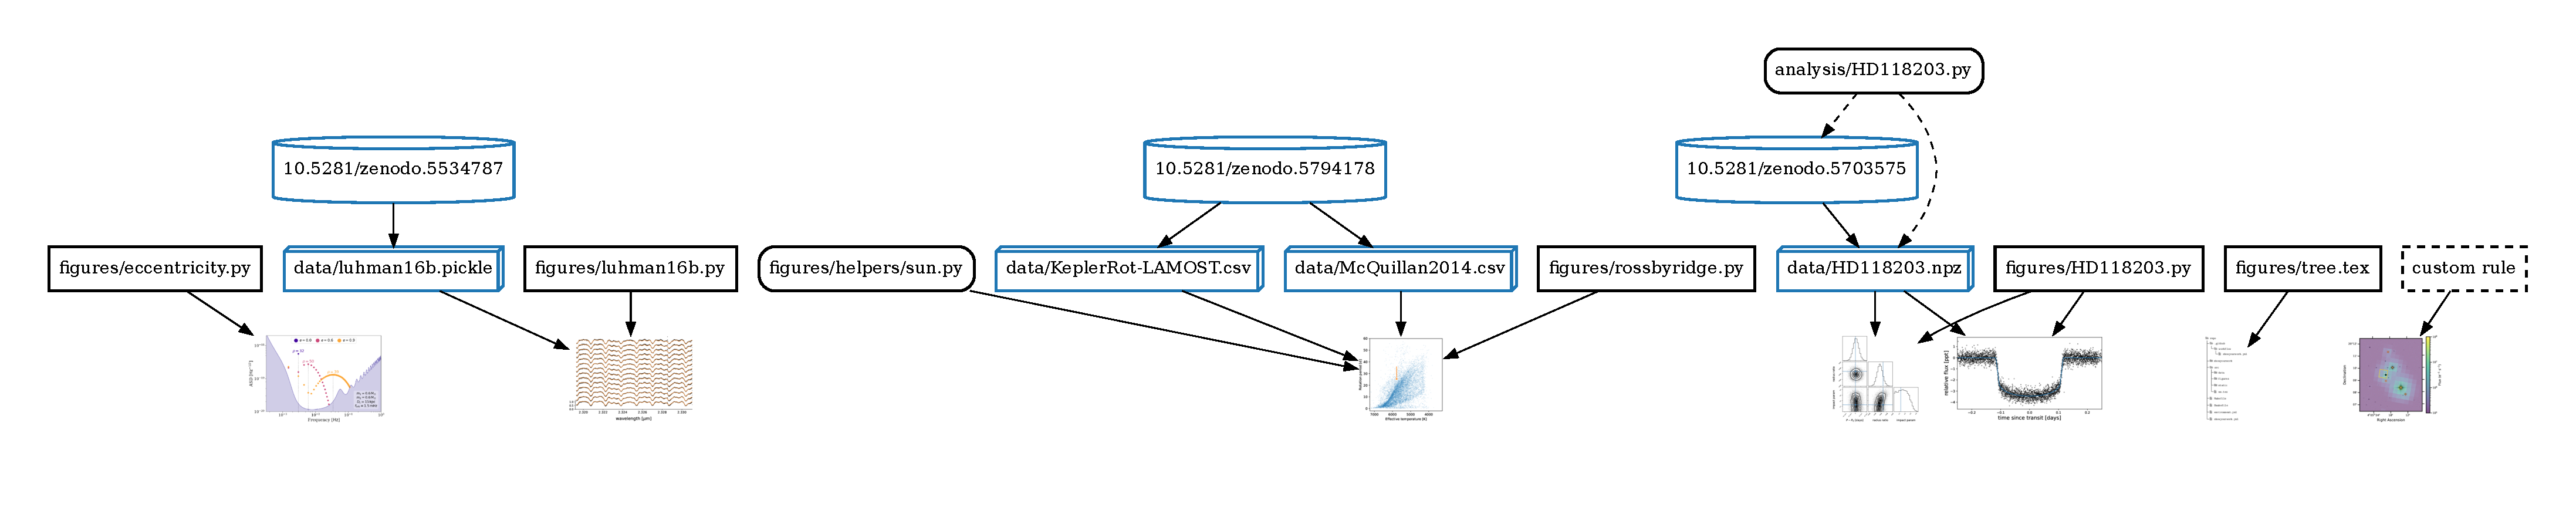
\includegraphics[width=\linewidth]{figures/dag.pdf}
        \caption{
            A directed acyclic graph (DAG) showing the build process for each of the (other) figures in this article. 
            Figure scripts are represented by black rectangles; helper scripts (such as ones imported by figure scripts or used in dataset generation) are similar, but have rounded edges.
            Blue cylinders correspond to Zenodo records; blue boxes correspond to datasets.
        }
        \label{fig*:dag}
    \end{centering}
\end{figure*}

\subsection{The \texttt{Snakefile}}
\label{sec:Snakefile}
%
\begin{minipage}{\linewidth}
\lstinputlisting[
    style=Snakefile
]
{../Snakefile}
\end{minipage}

\subsection{The \texttt{showyourwork.yml} file}
\label{sec:showyourworkyml}
%
\begin{minipage}{\linewidth}
\lstinputlisting[
    style=yaml
]
{../showyourwork.yml}
\end{minipage}

\subsection{The \texttt{environment.yml} file}
\label{sec:environmentyml}
%
\begin{minipage}{\linewidth}
\lstinputlisting[
    style=yaml
]
{../environment.yml}
\end{minipage}

\bibliography{bib}

\end{document}
